% Appendix B
% https://tex.stackexchange.com/questions/152829/how-can-i-highlight-yaml-code-in-a-pretty-way-with-listings

% \newgeometry{
% 	a4paper,
% 	top=21mm,
% 	bottom=11mm,
% 	inner=24mm,
% 	outer=9mm,
% } %bindingoffset=.5cm

%\newgeometry{
%	a4paper, inner=1.9cm, outer=1.9cm, bindingoffset=1.3cm, top=1.5cm, bottom=1.5cm, 
%} %bindingoffset=.5cm



\chapter{Implementation Details} % Main appendix title

A main goal of this thesis is to provide a code base that makes it as simple as possible to get started with \gencite{Derrac2015} algorithm to derive rudimentary conceptual spaces for any kind of dataset. In order to achieve this, documenting some implementation details and design decisions is crucial.
% TODO: something a la "es ist aber zu detailliert für den hauptteil und zerstört den lesefluss, deswegen ist der aufbau halt so dass der Hauptteil/der methods-section sich möglichst kurz fasst, wie halt die methods-section von nem Paper, und ebendieser appendix für diejenigen gedacht ist die den spezifischen Algorithmus genauer wissen wollen ODER den code nutzen wollen ODER sich einfach fragen warum dinge so sind wie sie sind. Also I HAVE to cite some of the used techniques as per their licences.
This appendix goes into more detail for selected components of the algorithm.

\label{AppendixB} 

\section{Algorithm Implementation Details}

\subsection*{Preprocessing\arrowref{sec:algo_preproc}}

\subsubsection*{Language-Detection and Translation}
\label{ap:translating}

To check the languages of the entities, the \codeother{langdetect}\footnote{\url{https://pypi.org/project/langdetect/}, \textcite{nakatani2010langdetect}} library is used, which is a direct port of a java library that claims to have 99.8\% accuracy on longer texts \cite{nakatani2010langdetect}. 

Depending on the translation-policy, it is possible to either take only those entities of the demanded language, ignore it and consider all entities in their original language, or enforce the demanded language by translating all entities from their original language to the demanded one. The accompaning code for this thesis contains extensive code to do that using the \emph{Google Cloud Translation API}\footnote{\url{https://cloud.google.com/translate}}. Many descriptions of the Siddata-dataset were translated using this technique\footnote{As, however, only 500.000 characters per google-account and month can be translated \href{https://cloud.google.com/translate/pricing}{free of charge}, the translation-process for the descriptions is still in progress.}. As of now, Google's Cloud Translation Service uses an embedding-based neural model of a hybrid architecture that has a transformer encoder, followed by an RNN decoder \cite{Chen2018}. All of the languages detected in the Siddata-dataset are supported by the system - translating between the languages German, English and Spanish, which make up more than 99 percent of the Siddata-descriptions, is what the system is particularly optimized for. 
% \todoparagraph{write short about their percentage, bleu score etc}

% \includeMD{pandoc_generated_latex/6_1_implementationdetails}

\subsection*{Candidate Extraction\arrowref{sec:extract_cands}}

\subsubsection*{KeyBERT}
\label{ap:details_keybert}

The \emph{KeyBERT}-algorithm\footnote{\label{fnote:keybertgibhut}\fullcite{MaartenGr2021}} \cite{grootendorst2020keybert} is one of the techniques used to select phrases of the text-corpus as candidates for feature-directions. 

KeyBERT is a keyword-extraction technique \q{that leverages BERT embeddings to create keywords and keyphrases that are most similar to a document}\footnoteref{fnote:keybertgibhut}. \Gls{bert} is a neural language representation model that is able to embed both words and documents. Its embeddings are obtained by training a multi-layer bidirectional transformer encoder \gls{ann} architecture on a task in which a masked word must be predicted from the its bidirectional context as well subsequent fine-tuning tasks \cite{Devlin2019}. To extract keywords, the KeyBERT algorithm embeds both the document as well as its containing \glspl{ngram} of a configurable length using BERT and returns those phrases whose embedding ist most similar to the document-embedding according to the cosine-similiarity\footnoteref{fnote:keybertgibhut}.

The KeyBERT-model was incorporated to extract key-phrases for this codebase in two ways: 

\paragraph{KeyBERT-original} runs the algorithm on the unprocessed original texts. This is reasonable, as this is what BERT-embeddings are trained on, however it has the disadvantage that it requires a lot of post-processing to match the extracted phrases to the processed descriptions (which \eg may contain only lemmas or have their \glspl{stopword} removed)
\paragraph{KeyBERT-preprocessed} alleviates this problems by running the algorithm on already preprocessed texts. This may however lead to worse results, as the algorithm was trained on unprocessed natural sentences.

In practice, though both variants extracted different phrases, the results for either of the technqiues did not differ significantly.


\subsection*{Candidate Filtering}
\label{ap:algo_filter}



\begin{figure}[H]
	\begin{center}
	  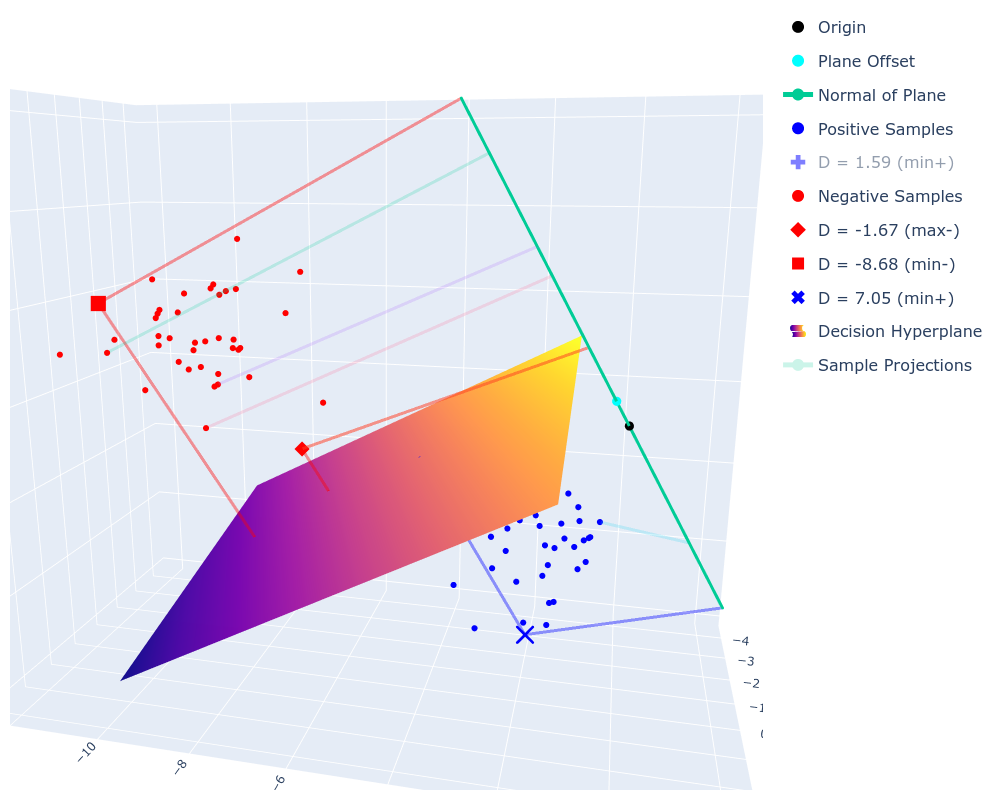
\includegraphics[width=.9\textwidth]{3dplot_hyperplane_and_orthogonal}
	  \caption[Visual representation of the hyperplane of an SVM splitting a dataset.]{ \label{fig:3d_hyperplane_ortho} Visual representation of the Hyperplane of a Support-Vector-Machine splitting a dataset, as well as it's orthogonal and the orthogonal projection of a set of samples onto the plane. For an interactive version of this plot, visit  {\small \url{https://nbviewer.org/github/cstenkamp/derive_conceptualspaces/blob/main/notebooks/text_referenced_plots/hyperplane_orthogonal_3d.ipynb?flush_cache}}}
	\end{center}
\end{figure}


\begin{table}[H]
    \centering
    \resizebox{\textwidth}{!}{%
    \begin{tabular}{llllll}
    \textbf{Long}                    & \textbf{Short} & \textbf{Data} & \textbf{Quantifications} & \textbf{Distances} & \textbf{Comments}                \\ \midrule
    rank2rank\_dense          & r2r-d          & all           & Dense-Ranked           & Dense-Ranked     &                                  \\
    rank2rank\_min            & r2r-min        & all           & Min-Ranked               & Dense-Ranked     &                                  \\
    bin2bin                   & b2b            & all           & Binary                   & Binary             & Disregards rankings              \\
    digitized &
      dig &
      all &
      Digitized &
      Digitized &
      \begin{tabular}[c]{@{}l@{}}10 bins. Positions decided by np.histogram\_bin\_edges \\ from min and max of all data \end{tabular} \\
    count2rank\_onlypos       & c2r+           & positive      & Unchanged                & Dense-Ranked     & Only for Count as Quantification \\
    rank2rank\_onlypos\_dense & r2r+d          & positive      & Dense-Ranked           & Dense-Ranked     &                                  \\
    rank2rank\_onlypos\_min   & r2r+min        & positive      & Min-Ranked               & Min-Ranked         &                                  \\
    rank2rank\_onlypos\_max   & r2r+max        & positive      & Max-Ranked               & Max-Ranked         &                                  \\
    digitized\_onlypos\_1 &
      dig+1 &
      positive &
      Digitized &
      Digitized &
      \begin{tabular}[c]{@{}l@{}}10 bins. Positions by np.histogram\_bin\_edges \\ from min and max of all data\end{tabular} \\
    digitized\_onlypos\_2 &
      dig+2 &
      positive &
      Digitized &
      Digitized &
      \begin{tabular}[c]{@{}l@{}}10 bins. Positions by np.histogram\_bin\_edges \\ from min and max of all positive data\end{tabular}
    \end{tabular}%
    }
    \slcaption{Different values of calculating Cohen's Kappa score. Dense means: if there are 14.900 zeros, the next is a 1.
    Min means: if there are 14.900 zeros, the next one is a 14.901.
    Max means: if there are 14.900 zeros, they all get the label 14.900.
    These scores are weighted.}
    \label{tab:kappa_measures}
\end{table}


\section{Other Algorithms}

\subsection{Semantic Knowledge Bases}

Lexical databases of semantic relations between words, the most famous of which being WordNet,\footnote{\url{https://wordnet.princeton.edu/}} link words in a graph that encodes explicit semantic relations like synonyms and hyponyms (subtypes/ \emph{is-a}-relationships). While neural %TODO: nicht neural, aber halt data-driven? naja das was word2vec undso sind... by-context-created/trained...?! similarity-based? -> DISTRIBUTIONAL MODELS (ones trained from the co-occurrence patterns of temrs)
embeddings may encode similar information implicitly, when relying on dictionary-based word encodings they are an important tool when using classical linguistic techniques. For the developed algorithm, the information how many hyponyms of a candidate word for a semantic direction %TODO: did I explain the algorithm well enough before this to throw this much information at the reader?!
occur in its corresponding text-corpus can be highly relevant. To do that, WordNet \cite{Miller1995} and it's German equivalent, GermaNet \cite{hamp-feldweg-1997-germanet,Henrich},\footnote{\url{https://uni-tuebingen.de/fakultaeten/philosophische-fakultaet/fachbereiche/neuphilologie/seminar-fuer-sprachwissenschaft/arbeitsbereiche/allg-sprachwissenschaft-computerlinguistik/ressourcen/lexica/germanet-1/}} are used in the respective step.


\subsection{Faculty-Classifier}
\label{sec:faculty_classifier}

As one of the evaluations is to compare the results of classifiers based on the algorithm here with a powerful classification algorithm, a neural network that classifies the faculty of a course in the Siddata-Dataset was also implemented. The implementation for that will not be elaborated upon except %that it is available at \todoparagraph{Link to the repo}, it relies on sacred, %\footnote{\todoparagraph{link to sacred, note that to get the results like done here you'll need a MongoDB in a docker container, see this link}} 
that it uses Google's `universal-sentence-encoder-multilingual` in Version 3 (linear in textlength, thus managable time and space requirements) plus a few classification layers ontop. The encoder is trained \q{on a number of natural language prediction tasks that require modeling the meaning of word sequences rather than just individual words},\footnote{Quote from their description at \urlx{https://tfhub.dev/google/collections/universal-sentence-encoder/1} \acc{03}{25} } aimed being the base for architectures for many NLP tasks through the usage of sentence embeddings \cite{Guo}. It was trained on with a train-test-split of 90/10 (the results being consitent through sampled cross-validation)


Another purpose of the classifier is to check if it is anyhow possible to extract meaningful information from the descriptions: If it is possible to train a classifier on the data that can reasonably predict a qualitative feature, there is enough structure in the data such that the algorithm we are about to produce can work. Also, we have a lower bound for useful data: we can just throw away data that cannot be classified.

% #########################################################################################################################################################################################################################################################################################################################################################################################################################################################################################################################################################################################################################################################################################################################################################################################################################################################

% \section{Used Software}

% \includeMD{pandoc_generated_latex/6_2_usedsoftware}

% #########################################################################################################################################################################################################################################################################################################################################################################################################################################################################################################################################################################################################################################################################################################################################################################################################################################################

\section{Configurations to run \cite{Derrac2015, Ager2018}}
\label{ap:yamls_for_origalgos}

% \vspace{-0.8cm}

% \lstinputlisting[language=, firstline=29]{codes/dqn.txt}

\subsection{\textcite{Derrac2015}}
\label{ap:yaml_for_derrac}

\begin{lstlisting}[language=yaml, caption={YAML for \textcite{Derrac2015}}]
    pp_components:          mfautcsdp
    quantification_measure: ppmi
    dissim_measure:         norm_ang_dist
    embed_algo:             mds
    embed_dimensions:       [20, 50, 100, 200]
    extraction_method:      pp_keybert
    max_ngram:              5                   
    dcm_quant_measure:      count
    classifier:             SVM
    classifier_succmetric:  [kappa_count2rank_onlypos, kappa_rank2rank_onlypos_min] 
    prim_lambda:            0.5
    sec_lambda:             0.1
    __perdataset__:
      placetypes:
        extraction_method:  all 
        pp_components:      none
\end{lstlisting}

\subsection{\textcite{Ager2018}}

\input{pandoc_generated_latex/ZZ_listingreplacement_ager}

% \begin{lstlisting}[language=yaml, caption={YAML for \textcite{Ager2018}}]
%     max_ngram:              1
%     classifier_succmetric:  [cohen_kappa, accuracy, ndcg]
%     dcm_quant_measure:      ppmi    
% \end{lstlisting}


% \todo 


% \subsection{\textcite{Alshaikh2020}}
% \begin{lstlisting}[language=yaml, caption={YAML for \textcite{Alshaikh2020}}]
%     TODO: do
% \end{lstlisting}
